% Chapter 5

\chapter{Quantum Classifiers And Decision Boundaries} % Main chapter title

\label{chapter:quantum_classifiers_decision_boundaries}
\todo{explain ansatz and why and also quantum classifier in general}
%----------------------------------------------------------------------------------------
To analyze the expressiveness of quantum circuits contour plots are used to show the decision boundaries of trained quantum classifiers.\\
The following experiments\todo{use figures and reference them here, so that it is 100\% clear what is meant} show three different artificial problems consisting of two moons (make\_moons), circle shaped (make\_circles) and linearly separable data (make\_classfication) from top to bottom. All data sets have only two classes (binary) and 100 data points. The data given to the quantum classifiers has been scaled to $\mathrm{[-1,1]}$. The classifier which receives the measured output of the quantum circuit is defined as follows:
\hfill \break

$f : X \rightarrow\mathbb{R}$. The quantum classifier assigns a binary label to $x$ according to the threshold rule:

\begin{equation}
    \centering
    \begin{split}
    y =
        \left\{\begin{matrix}
            -1\ if\ f(x) < \tau ,\\
            1\ if\ f(x) \geq \tau
        \end{matrix}\right.
    \end{split}
    \label{equation:classifier_definition}
\end{equation}

with $\tau\in\mathbb{R}$ and $\tau$ is equal to zero.\todo{$\tau$ equal to zero?}\\
\hfill \break 
Data was splitted with $75\%$ being used for training and $25\%$ for testing. The \href{https://www.pennylane.ai}{Pennylane.ai} framework has been used with the \href{https://pennylane.readthedocs.io/en/stable/code/api/pennylane.devices.default_qubit.html#module-pennylane.devices.default_qubit}{\code{default.qubit}} simulator. Optimization is done with the \href{https://pennylane.readthedocs.io/en/stable/code/api/pennylane.NesterovMomentumOptimizer.html}{\code{NesterovMomentumOptimizer}} optimizer.

\clearpage
\subsection{Single Qubit Circuits}
\label{subsection:single_qubit_circuits}

In this subsection two single qubit quantum classifiers with feature embedding between weights and a total count of six weights a have been trained. For comparison there is also a Multi-layer Perceptron classifier (sklearn neureal network \href{https://scikit-learn.org/stable/modules/generated/sklearn.neural_network.MLPClassifier.html}{\code{MLPClassifier}}) in the plots with the same iteration count as the quantum classifiers. Figure \ref{fig:SingleQubitClassifiers_50Iterations} has a iteration count of 50, figure \ref{fig:SingleQubitClassifiers_200Iterations} shows 200 iterations and the last figure \ref{fig:SingleQubitClassifiers_400Iterations} shows the classifiers after 400 iterations. The quantum classifiers score shows the latest iteration of the validation set accuracy while the score for the \code{MLPClassifier} is the mean accuracy.\\
\\

\begin{figure}[h!]
    \centering
    
    \begin{subfigure}{1.0\textwidth}
        \centering
        \scalebox{0.66}{
            \Qcircuit @C=1.0em @R=0.2em @!R { \\
            	 	\nghost{ {q}_{0} :  } & \lstick{ {q}_{0} :  } & \gate{\mathrm{R_Y}\,(\mathrm{\color{magenta}x_0})} & \gate{\mathrm{R_Z}\,(\mathrm{\color{gray}w_0})} & \gate{\mathrm{R_Y}\,(\mathrm{\color{gray}w_1})} & \gate{\mathrm{R_Z}\,(\mathrm{\color{gray}w_2})} & \gate{\mathrm{R_Y}\,(\mathrm{\color{magenta}x_1})} & \gate{\mathrm{R_Z}\,(\mathrm{\color{gray}w_3})} & \gate{\mathrm{R_Y}\,(\mathrm{\color{gray}w_4})} & \gate{\mathrm{R_Z}\,(\mathrm{\color{gray}w_5})} & \qw & \qw\\ 
            \\ }
        }
        \caption{\textbf{Quantum Circuit classifier 1} with only $\mathrm{RY}$ and $\mathrm{RZ}$ gates using 6 weights and two input features $\mathrm{x_0}$, $\mathrm{x_1}$ }
        \label{fig:single_qubit_circuit_1}
    \end{subfigure}
    \\[2ex]
    \begin{subfigure}{1.0\textwidth}
        \centering
        \scalebox{0.66}{
            \Qcircuit @C=1.0em @R=0.2em @!R { \\
            	 	\nghost{ {q}_{0} :  } & \lstick{ {q}_{0} :  } & \gate{\mathrm{R_Y}\,(\mathrm{\color{magenta}x_0})} & \gate{\mathrm{R_Z}\,(\mathrm{\color{gray}w_0})} & \gate{\mathrm{R_Y}\,(\mathrm{\color{gray}w_1})} & \gate{\mathrm{R_Z}\,(\mathrm{\color{gray}w_2})} & \gate{\mathrm{R_X}\,(\mathrm{\color{magenta}x_1})} & \gate{\mathrm{R_Z}\,(\mathrm{\color{gray}w_3})} & \gate{\mathrm{R_Y}\,(\mathrm{\color{gray}w_4})} & \gate{\mathrm{R_Z}\,(\mathrm{\color{gray}w_5})} & \qw & \qw\\ 
            \\ }
        }
        \caption{\textbf{Quantum Circuit classifier 2} with $\mathrm{RY}$, $\mathrm{RZ}$ gates and a $\mathrm{RX}$ gate using also 6 weights and two input features $\mathrm{x_0}$, $\mathrm{x_1}$ }
        \label{fig:single_qubit_circuit_2}
    \end{subfigure}
    
    \caption{Single qubit quantum circuits referring to \textbf{Quantum Circuit classifier 1} and \textbf{Quantum Circuit classifier 2} in figures \ref{fig:SingleQubitClassifiers_50Iterations}, \ref{fig:SingleQubitClassifiers_200Iterations} and \ref{fig:SingleQubitClassifiers_400Iterations}.}
    \label{fig:single_qubit_circuits}
\end{figure}

% Contour plots
\begin{figure}[h!]
    \centering
    
    \begin{subfigure}{1.0\textwidth}
        \centering
        \scalebox{0.27}{
            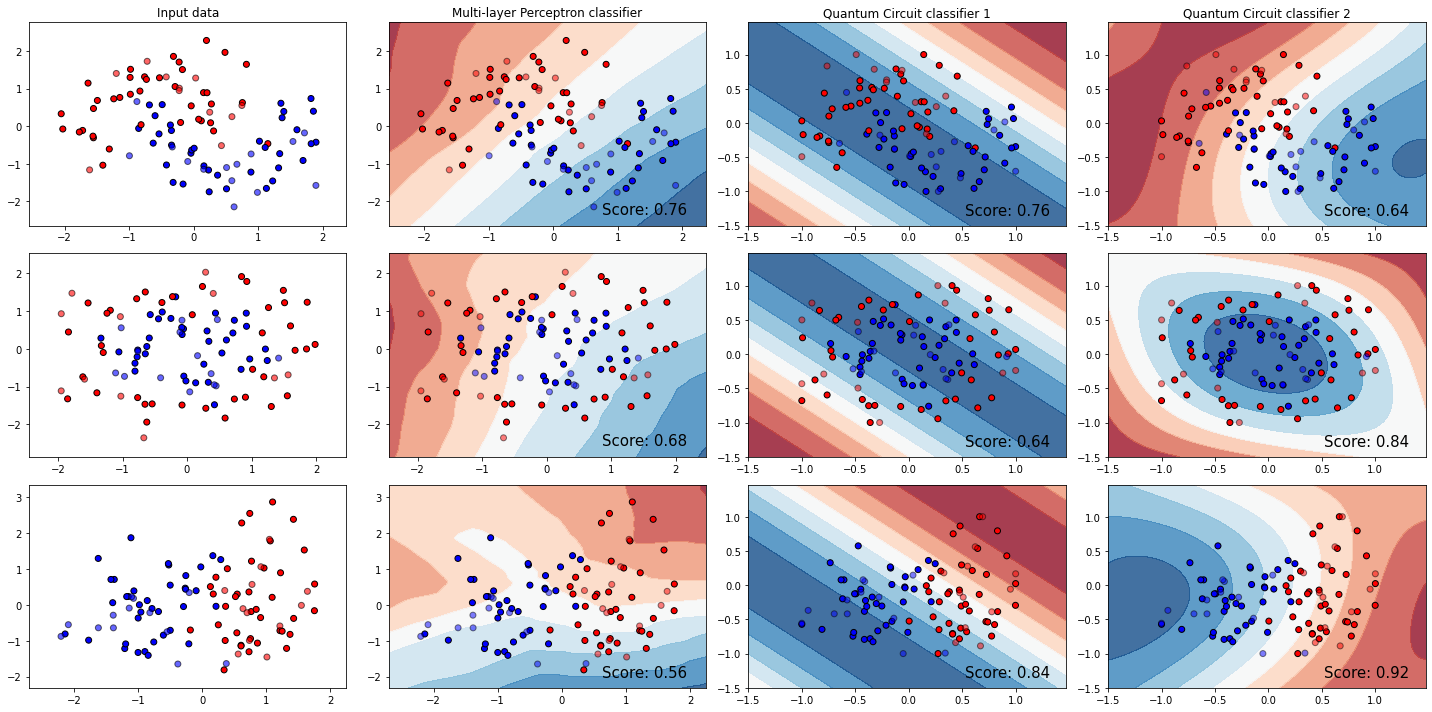
\includegraphics{Appendices/chapter_5/SingleQubitClassifiers_50Iterations.png}
        }
        \caption{Decision boundary and score comparison between Multi-layer Perceptron classifier, Quantum Circuit classifier 1 and Quantum Circuit classifier 2, limited to \textbf{50 iterations} for all classifiers using \textbf{single qubit quantum circuits}.}
        \label{fig:SingleQubitClassifiers_50Iterations}
    \end{subfigure}
    \\[2ex]
    \begin{subfigure}{1.0\textwidth}
        \centering
        \scalebox{0.27}{
            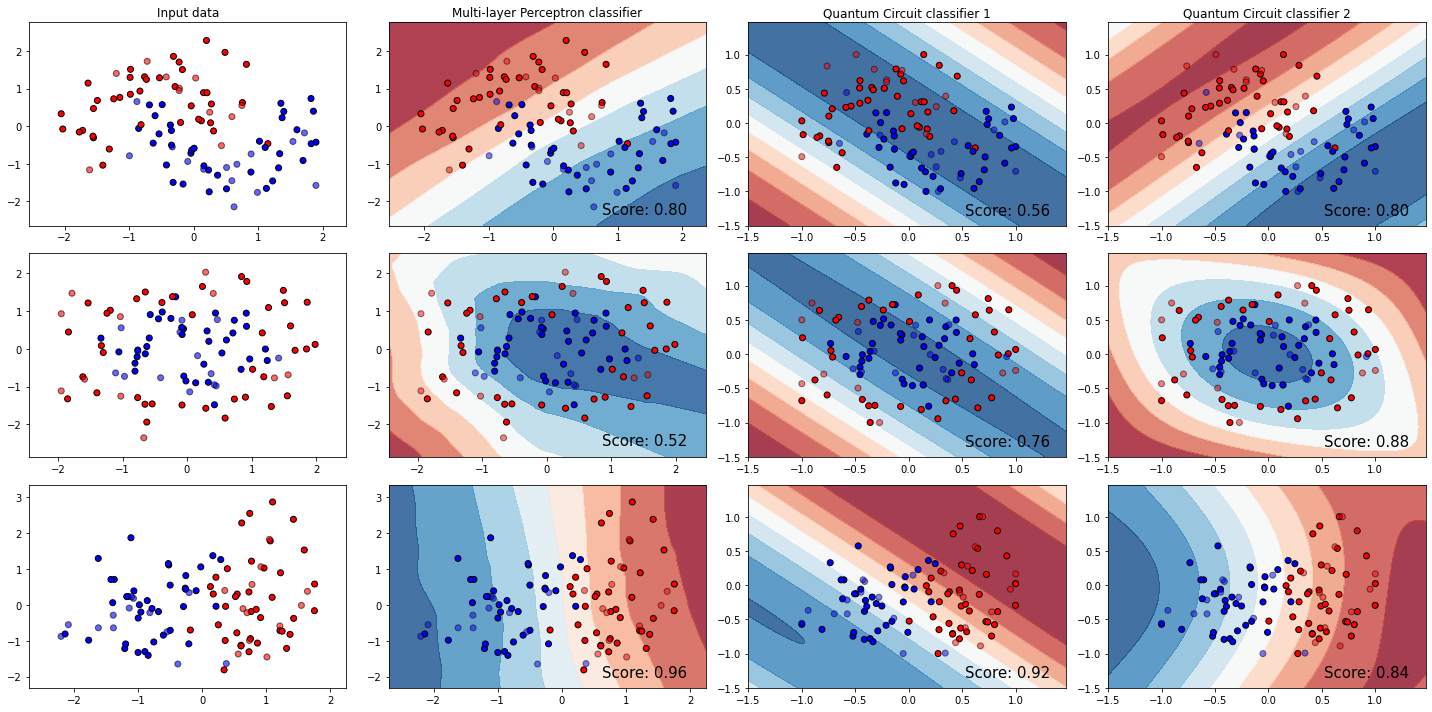
\includegraphics{Appendices/chapter_5/SingleQubitClassifiers_200Iterations.png}
        }
        \caption{Decision boundary and score comparison between Multi-layer Perceptron classifier, Quantum Circuit classifier 1 and Quantum Circuit classifier 2, limited to \textbf{200 iterations} for all classifiers using \textbf{single qubit quantum circuits}.}
        \label{fig:SingleQubitClassifiers_200Iterations}
    \end{subfigure}
    \\[2ex]
    \begin{subfigure}{1.0\textwidth}
        \centering
        \scalebox{0.27}{
            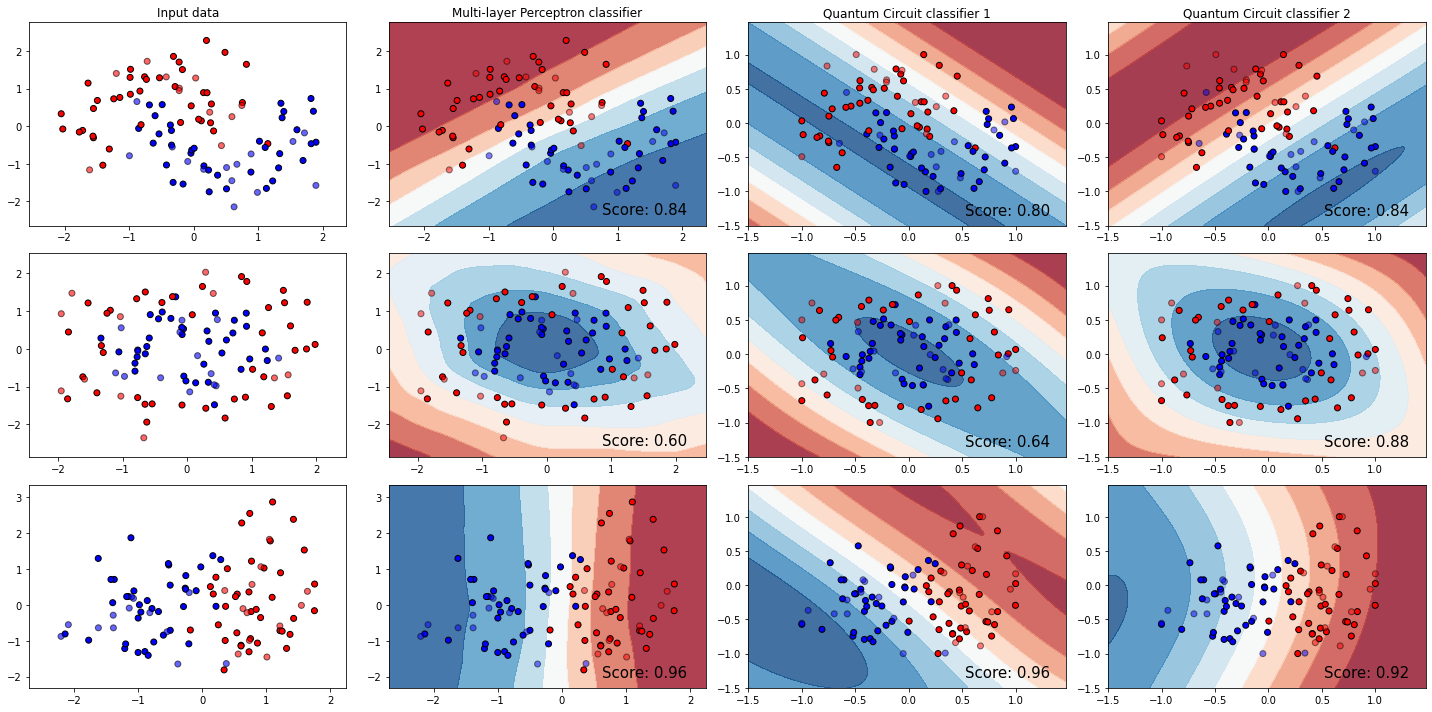
\includegraphics{Appendices/chapter_5/SingleQubitClassifiers_400Iterations.png}
        }
        \caption{Decision boundary and score comparison between Multi-layer Perceptron classifier, Quantum Circuit classifier 1 and Quantum Circuit classifier 2, limited to \textbf{400 iterations} for all classifiers using \textbf{single qubit quantum circuits}.}
        \label{fig:SingleQubitClassifiers_400Iterations}
    \end{subfigure}
    
\end{figure}

\clearpage
\subsection{Two qubit circuits}
\label{subsection:two_qubit_circuits}

In this subsection three two qubit quantum classifiers with angle embedding and a total count of six weights a have been trained. For comparison there is also a Multi-layer Perceptron classifier (sklearn neureal network \href{https://scikit-learn.org/stable/modules/generated/sklearn.neural_network.MLPClassifier.html}{MLPClassifier}) in the plots with the same iteration count as the quantum classifiers. Figure \ref{fig:2QubitClassifiers_50Iterations} has a iteration count of 50, figure \ref{fig:2QubitClassifiers_200Iterations} shows 200 iterations and the last figure \ref{fig:2QubitClassifiers_400Iterations} shows the classifiers after 400 iterations. The quantum classifiers score shows the latest iteration of the validation set accuracy while the score for the \code{MLPClassifier} is the mean accuracy.\\
\\

\begin{figure}[!h]
    \centering
    
    \begin{subfigure}{1.0\textwidth}
        \centering
        \scalebox{0.66}{
            \Qcircuit @C=1.0em @R=0.2em @!R { \\
            	 	\nghost{ {q}_{0} :  } & \lstick{ {q}_{0} :  } & \gate{\mathrm{H}} & \gate{\mathrm{R_Y}\,(\mathrm{\color{magenta}x_0})} & \ctrl{1} & \gate{\mathrm{R_Z}\,(\mathrm{\color{gray}w_0})} & \gate{\mathrm{R_Y}\,(\mathrm{\color{gray}w_1})} & \gate{\mathrm{R_Z}\,(\mathrm{\color{gray}w_2})} & \ctrl{1} & \qw & \qw\\ 
            	 	\nghost{ {q}_{1} :  } & \lstick{ {q}_{1} :  } & \gate{\mathrm{H}} & \gate{\mathrm{R_Y}\,(\mathrm{\color{magenta}x_1})} & \targ & \gate{\mathrm{R_Z}\,(\mathrm{\color{gray}w_3})} & \gate{\mathrm{R_Y}\,(\mathrm{\color{gray}w_4})} & \gate{\mathrm{R_Z}\,(\mathrm{\color{gray}w_5})} & \targ & \qw & \qw\\ 
            \\ }
        }
        \caption{\textbf{Quantum Circuit classifier 1} with starting Hadamard ($\mathrm{H}$) gates and angle embedding using a $\mathrm{RY}$ gates entangled with a $\mathrm{CX}$ gate followed by multiple $\mathrm{RY}$ and $\mathrm{RZ}$ rotation gates containing six weights in total, entangled with a final $\mathrm{CX}$ gate}
        \label{fig:two_qubit_circuit_1}
    \end{subfigure}
    \\[2ex]
    \begin{subfigure}{1.0\textwidth}
        \centering
        \scalebox{0.66}{
            \Qcircuit @C=1.0em @R=0.2em @!R { \\
            	 	\nghost{ {q}_{0} :  } & \lstick{ {q}_{0} :  } & \gate{\mathrm{H}} & \gate{\mathrm{R_Y}\,(\mathrm{\color{magenta}x_0})} & \gate{\mathrm{R_X}\,(\mathrm{\color{magenta}x_1})} & \ctrl{1} & \gate{\mathrm{R_Z}\,(\mathrm{\color{gray}w_0})} & \gate{\mathrm{R_Y}\,(\mathrm{\color{gray}w_1})} & \gate{\mathrm{R_Z}\,(\mathrm{\color{gray}w_2})} & \ctrl{1} & \qw & \qw\\ 
            	 	\nghost{ {q}_{1} :  } & \lstick{ {q}_{1} :  } & \gate{\mathrm{H}} & \qw & \qw & \targ & \gate{\mathrm{R_Z}\,(\mathrm{\color{gray}w_3})} & \gate{\mathrm{R_Y}\,(\mathrm{\color{gray}w_4})} & \gate{\mathrm{R_Z}\,(\mathrm{\color{gray}w_5})} & \targ & \qw & \qw\\ 
            \\ }
        }
        \caption{\textbf{Quantum Circuit classifier 2} differs from \textbf{Quantum Circuit classifier 1} \ref{fig:two_qubit_circuit_1} in terms of angle embedding using a $\mathrm{RY}$ and a $\mathrm{RX}$ gate to encode both features $x_0$, $x_1$ on the first qubit $q_0$ instead of using both qubits}
        \label{fig:two_qubit_circuit_2}
    \end{subfigure}
    \\[2ex]
    \begin{subfigure}{1.0\textwidth}
        \centering
        \scalebox{0.66}{
            \Qcircuit @C=1.0em @R=0.2em @!R { \\
        	 	\nghost{ {q}_{0} :  } & \lstick{ {q}_{0} :  } & \gate{\mathrm{H}} & \gate{\mathrm{R_Y}\,(\mathrm{\color{magenta}x_0})} & \ctrl{1} & \gate{\mathrm{R_Z}\,(\mathrm{\color{gray}w_0})} & \gate{\mathrm{R_Y}\,(\mathrm{\color{gray}w_1})} & \gate{\mathrm{R_Z}\,(\mathrm{\color{gray}w_2})} & \ctrl{1} & \qw & \qw\\ 
        	 	\nghost{ {q}_{1} :  } & \lstick{ {q}_{1} :  } & \gate{\mathrm{H}} & \gate{\mathrm{R_X}\,(\mathrm{\color{magenta}x_1})} & \targ & \gate{\mathrm{R_Z}\,(\mathrm{\color{gray}w_3})} & \gate{\mathrm{R_Y}\,(\mathrm{\color{gray}w_4})} & \gate{\mathrm{R_Z}\,(\mathrm{\color{gray}w_5})} & \targ & \qw & \qw\\ 
            \\ }
        }
        \caption{\textbf{Quantum Circuit classifier 3} with starting Hadamard ($\mathrm{H}$) gates and angle embedding using a $\mathrm{RY}$ and a $\mathrm{RX}$ gate}
        \label{fig:two_qubit_circuit_3}
    \end{subfigure}
    
    \caption{Two qubit quantum circuits referring to the \textbf{Quantum Circuit classifier 1}, \textbf{Quantum Circuit classifier 2} and \textbf{Quantum Circuit classifier 3} in figures \ref{fig:2QubitClassifiers_50Iterations}, \ref{fig:2QubitClassifiers_200Iterations} and \ref{fig:2QubitClassifiers_400Iterations}.}
    \label{fig:two_qubit_circuits}
\end{figure}

% Contour plots
\begin{figure}[!h]
    \centering

    \begin{subfigure}{1.0\textwidth}
        \centering
        \scalebox{0.27}{
            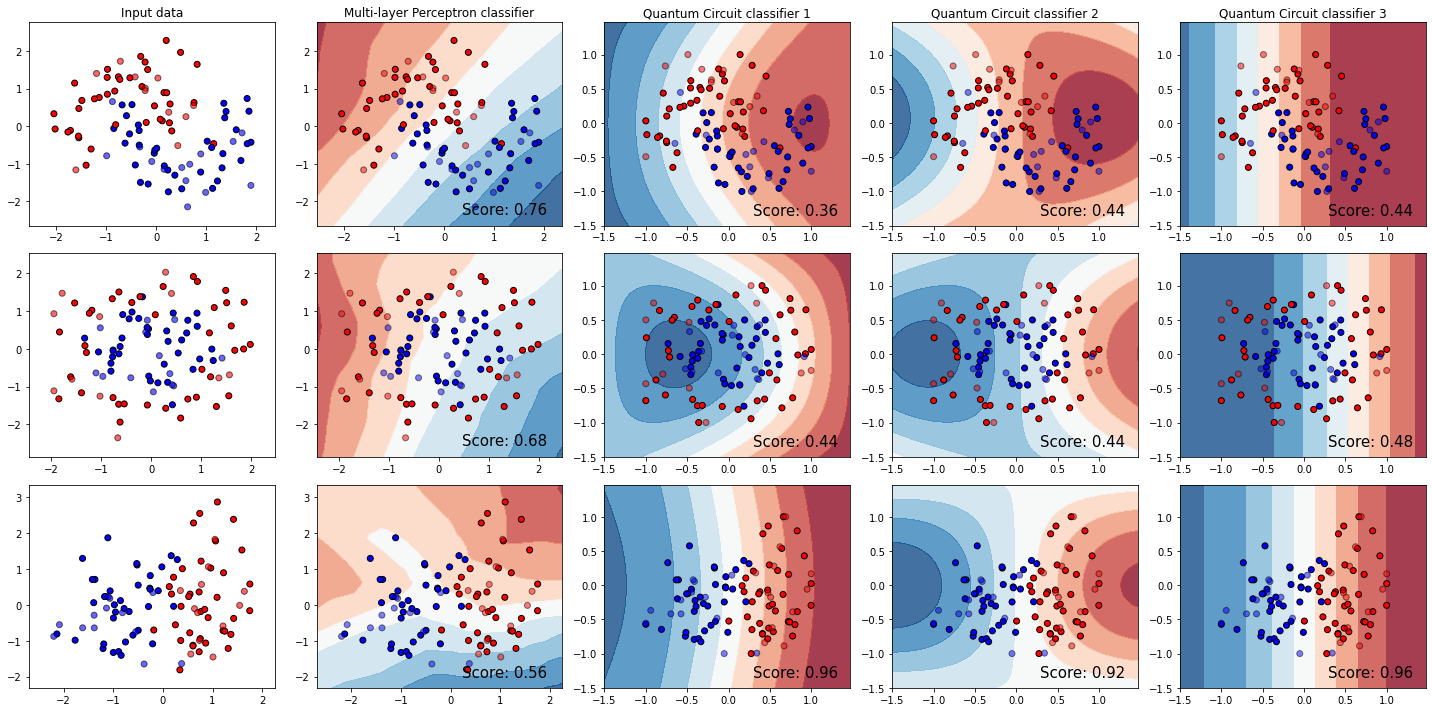
\includegraphics{Appendices/chapter_5/2QubitClassifiers_50Iterations.png}
        }
        \caption{Decision boundary and score comparison between Multi-layer Perceptron classifier, Quantum Circuit classifier 1 and Quantum Circuit classifier 2, limited to \textbf{50 iterations} for all classifiers using \textbf{two qubit quantum circuits}.}
        \label{fig:2QubitClassifiers_50Iterations}
    \end{subfigure}
    \\[2ex]
    \begin{subfigure}{1.0\textwidth}
        \centering
        \scalebox{0.27}{
            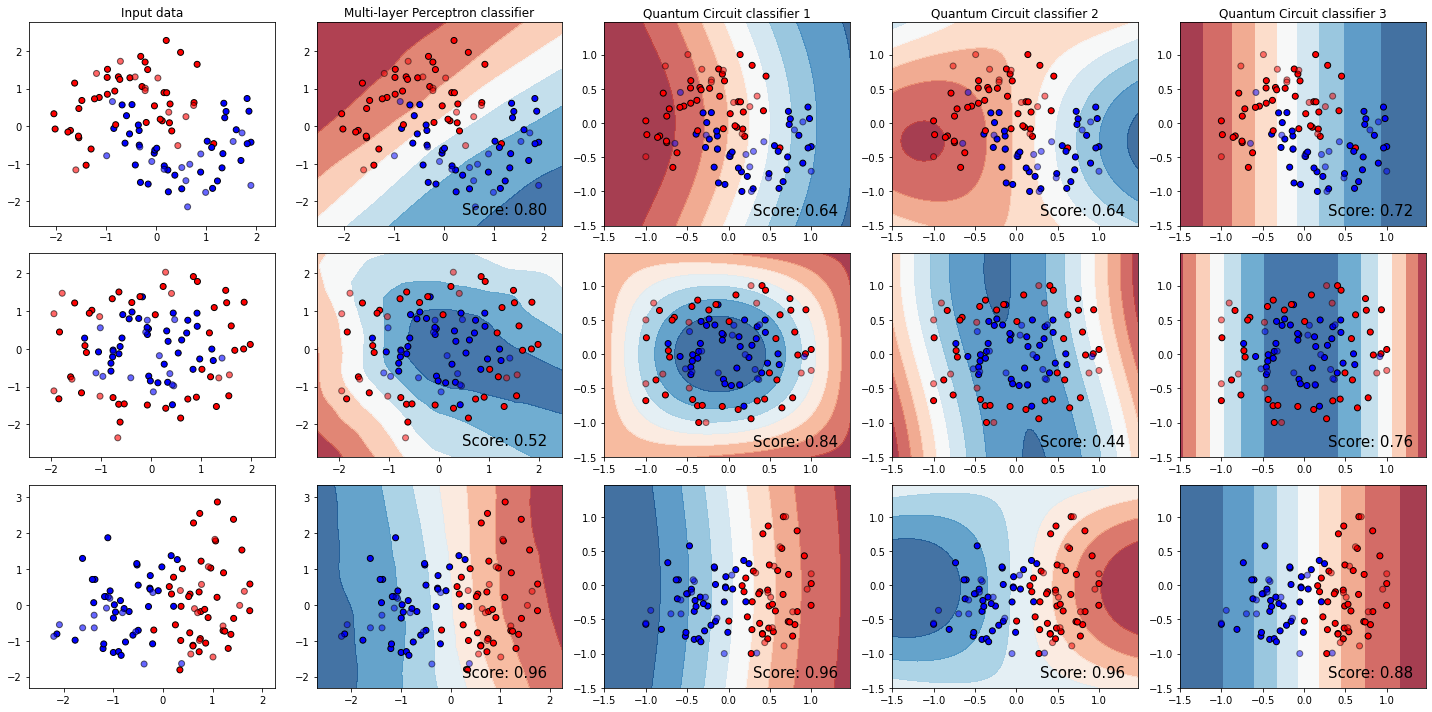
\includegraphics{Appendices/chapter_5/2QubitClassifiers_200Iterations.png}
        }
        \caption{Decision boundary and score comparison between Multi-layer Perceptron classifier, Quantum Circuit classifier 1 and Quantum Circuit classifier 2, limited to \textbf{200 iterations} for all classifiers using \textbf{two qubit quantum circuits}.}
        \label{fig:2QubitClassifiers_200Iterations}
    \end{subfigure}
    \\[2ex]
    \begin{subfigure}{1.0\textwidth}
        \centering
        \scalebox{0.27}{
            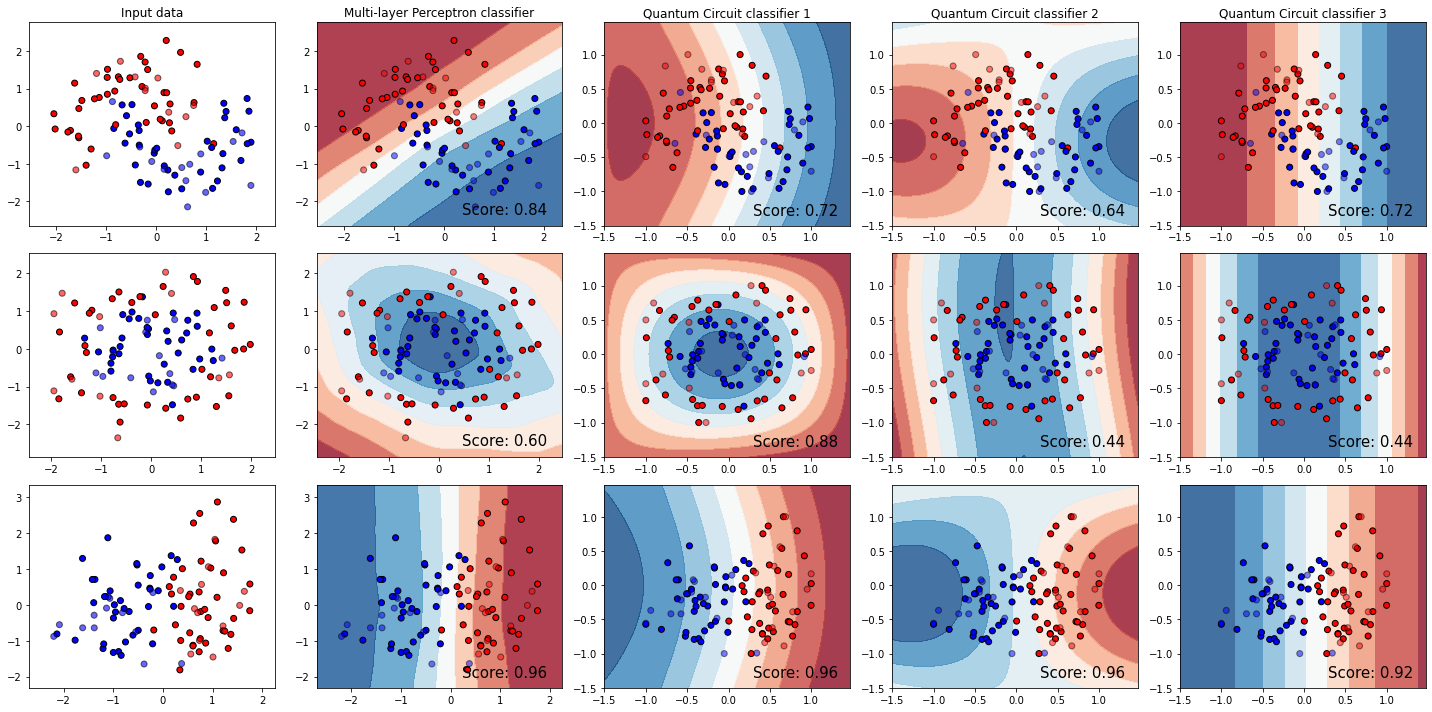
\includegraphics{Appendices/chapter_5/2QubitClassifiers_400Iterations.png}
        }
        \caption{Decision boundary and score comparison between Multi-layer Perceptron classifier, Quantum Circuit classifier 1, Quantum Circuit classifier 2 and Quantum Circuit classifier 3, limited to \textbf{400 iterations} for all classifiers using \textbf{two qubit quantum circuits}.}
        \label{fig:2QubitClassifiers_400Iterations}
    \end{subfigure}
\end{figure}

\clearpage
\section{Discussion}

\subsection{Single qubit classifiers}
Examining the single qubit classifier plots and comparing the quantum classifiers decision boundaries, it becomes obvious that the replacing of the $\mathrm{RY}$ gate in \textit{Quantum Circuit classifier 1} (\ref{fig:single_qubit_circuit_1}) with an $\mathrm{RX}$ gate in \textit{Quantum Circuit classifier 2} (\ref{fig:single_qubit_circuit_2}) for the feature $x_1$ enhanced the expressiveness of the \textit{Quantum Circuit classifier 2} in a very beneficial way, resulting in a much higher score over nearly all iteration counts.

Another interesting observation is that the \textit{Quantum Circuit classifier 1} consisting only of $\mathrm{RY}$ and $\mathrm{RZ}$ gates is able to adapt the weights to more and more resemble the data, mostly increasing the score with higher iterations but achieving this much slower than \textit{Quantum Circuit classifier 2}.

Comparing the linearly separable data (second and third row of figure \ref{fig:SingleQubitClassifiers_50Iterations}) between the \textit{Multi-layer Perceptron classifier} and \textit{Quantum Circuit classifier 2} with only 50 iterations, the \textit{Quantum Circuit classifier 2} outperforms the \textit{Multi-layer Perceptron classifier}, but the \textit{Multi-layer Perceptron classifier} is able to keep up again and over perform with more iterations as seen in figures \ref{fig:SingleQubitClassifiers_200Iterations} and \ref{fig:SingleQubitClassifiers_400Iterations}, at least for the linearly separable data.

\subsection{Two qubit classifiers}


\section{Conclusion}
Conclusion ...
